\documentclass{article}

\usepackage{amsmath}
\usepackage{amssymb}
\usepackage{amsthm}
\usepackage{mathpartir}
\usepackage{fontawesome5}
\usepackage{xcolor}
\usepackage{tikz}
\usepackage{amsmath}

\usetikzlibrary{arrows.meta,positioning}
\tikzset{graphnode/.style={draw,circle,inner sep=1.5pt,minimum size=18pt}}
\mprset{flushleft}

\newtheorem{theorem}{Theorem}
\newtheorem{lemma}[theorem]{Lemma}
\newtheorem{corollary}[theorem]{Corollary}
\newtheorem{definition}[theorem]{Definition}

\newcommand{\kw}[1]{\text{\textbf{#1}}}
\newcommand{\judge}[3]{#1 \vdash #2 : #3}
\newcommand{\Jud}[2]{\judge{\Gamma}{#1}{#2}}
\newcommand{\leqto}{\mathrel{\leq_{\mathrm{to}}}}
\newcommand{\leqin}{\mathrel{\leq_{\mathrm{in}}}}
\newcommand{\mode}[1]{\textsc{#1}}
\newcommand{\subtype}{\mathrel{\sqsubseteq}}
\newcommand{\Alias}[2]{#1 \mathrel{\underset{\text{alias}}{\rightsquigarrow}} #2}
\newcommand{\Lock}[2][]{\text{\faLock}_{#1}(#2)}

\newcommand{\Rel}[2]{\mathcal{R}_{#1}(#2)}
\newcommand{\Solve}[1]{\mathsf{solve}(#1)}
\newcommand{\Constraint}[1]{\mathcal{C}\!\left(#1\right)}
\newcommand{\RelSet}{\mathsf{Rel}}
\newcommand{\Cl}{\mathsf{Cl}}

\newcommand{\todo}[1]{\textcolor{red}{\textbf{TODO:} #1}}

\title{Relational Solver Notes}
\author{Jules Jacobs}
\date{\today}

\begin{document}

\maketitle

\section{Roadmap}

This document sketches the relational solver that accompanies the Mox type system notes.
The goal is to develop a mode solver that is powerful enough to handle the mode constraints produced by the type checker.

At a high level, we will develop a solver for binary constraints between modes.
We will first analyze a class of constraints that can be solved in polynomial time.
Then we will develop a more powerful solver that can handle that class of constraints.

\section{Constraint Language}

As a first step, assume we have a finite domain $V$ of values, and a set of binary relations $R_i \subseteq V \times V$.
Given a set of variables and asserted contraints between them, we want to determine if there exists a valuation of the variables that satisfies all the constraints.

In general this is a NP-complete problem: consider $V=\{0,1,2,\dots,k\}$ and $R_1 = \{ (a,b) \mid a \neq b \} \subseteq V \times V$.
Given a graph we can use this constraints to encode the $k$-coloring problem: we want to assign a color to each vertex such that no two adjacent vertices have the same color. The $k$-coloring problem is NP-complete, so this problem is also NP-complete.

However, certain classes of constraints can be solved in polynomial time. Consider the set of constraints $R_i = \{ (a,b) \mid b \geq a + i \} \subseteq V \times V$. Given a graph of variables and constraints, we can solve this problem in polynomial time using the Floyd-Warshall algorithm.

Equivalently, we can solve the problem by variable elimination: we take a variable $x$ and all adjacent constraints on it. We assert all transitive constraints (where $R_i$ composes with $R_j$ to produce $R_{i+j}$) and repeat until all variables are eliminated.
If, during this process, we ever see a constraint between a variable and itself with $i \neq 0$, then the constraints are unsatisfiable.

Why does this elimination strategy work for this class of constraints, but not for the general case, and in particular for the $k$-coloring problem with inequality constraints?

Consider a variable $x$ with:
\begin{itemize}
    \item a set of predecessors $a_1,a_2,a_3$ with $R_{i_1}(a_1,x), R_{i_2}(a_2,x), R_{i_3}(a_3,x)$ constraints on them,
    \item a set of successors $b_1,b_2$ with $R_{j_1}(x,b_1), R_{j_2}(x,b_2)$ constraints on them,
\end{itemize}
When eliminating $x$, we assert every transitive constraint $R_{i_p + j_q}(a_p,b_q)$ for $p \in \{1,2,3\}$ and $q \in \{1,2\}$:

\begin{figure}[ht]
  \centering
  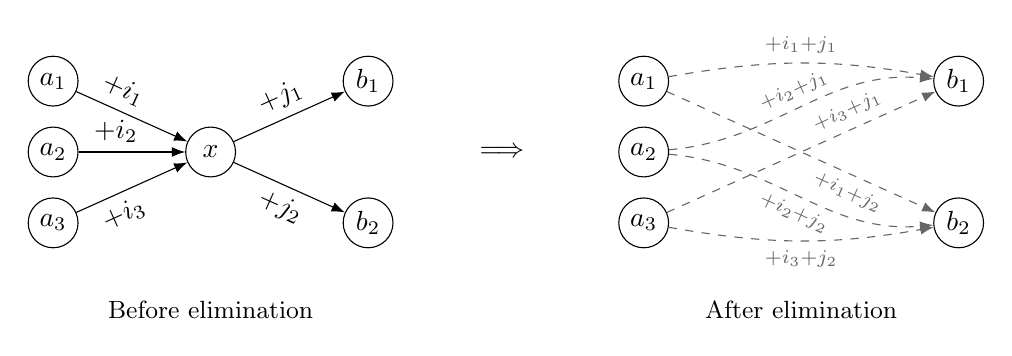
\begin{tikzpicture}[>=Latex]
    \begin{scope}[xshift=-2.5cm]
      \node[graphnode] (a1) at (0,0.9) {$a_1$};
      \node[graphnode] (a2) at (0,0) {$a_2$};
      \node[graphnode] (a3) at (0,-0.9) {$a_3$};
      \node[graphnode] (x)  at (2,0) {$x$};
      \node[graphnode] (b1) at (4,0.9) {$b_1$};
      \node[graphnode] (b2) at (4,-0.9) {$b_2$};

      \draw[->] (a1) -- node[pos=0.35,above,sloped] {$+i_1$} (x);
      \draw[->] (a2) -- node[pos=0.35,above] {$+i_2$} (x);
      \draw[->] (a3) -- node[pos=0.35,below,sloped] {$+i_3$} (x);

      \draw[->] (x) -- node[above,sloped] {$+j_1$} (b1);
      \draw[->] (x) -- node[below,sloped] {$+j_2$} (b2);

      \node[font=\small,align=center] at (2,-2) {Before elimination};
    \end{scope}

    \node at (3.2,0) {$\Longrightarrow$};

    \begin{scope}[xshift=5cm]
      \node[graphnode] (a1p) at (0,0.9) {$a_1$};
      \node[graphnode] (a2p) at (0,0) {$a_2$};
      \node[graphnode] (a3p) at (0,-0.9) {$a_3$};
      \node[graphnode] (b1p) at (4,0.9) {$b_1$};
      \node[graphnode] (b2p) at (4,-0.9) {$b_2$};

      \draw[dashed,->,black!60] (a1p) to[out=10,in=170] 
        node[pos=0.5,sloped,above,font=\scriptsize] {$+i_1{+}j_1$} (b1p);
      \draw[dashed,->,black!60] (a1p) --
        node[pos=0.7,sloped,below,font=\scriptsize] {$+i_1{+}j_2$} (b2p);

      \draw[dashed,->,black!60] (a2p) to[out=5,in=175]
        node[pos=0.5,sloped,above,font=\scriptsize] {$+i_2{+}j_1$} (b1p);
      \draw[dashed,->,black!60] (a2p) to[out=-5,in=-175]
        node[pos=0.5,sloped,below,font=\scriptsize] {$+i_2{+}j_2$} (b2p);

      \draw[dashed,->,black!60] (a3p) --
        node[pos=0.7,sloped,above,font=\scriptsize] {$+i_3{+}j_1$} (b1p);
      \draw[dashed,->,black!60] (a3p) to[out=-10,in=-170]
        node[pos=0.5,sloped,below,font=\scriptsize] {$+i_3{+}j_2$} (b2p);

      \node[font=\small,align=center] at (2,-2) {After elimination};
    \end{scope}
  \end{tikzpicture}
\end{figure}

I claim that if there is a solution for the neighboring variables that satisfies all of those transitive constraints, then there is a solution for $x$ that satisfies the original constraints: we can simply set $x$ to any value in the interval $\max(a_1 + i_1, a_2 + i_2, a_3 + i_3) \leq x \leq \min(b_1 + j_1, b_2 + j_2)$. This interval is guaranteed to be non-empty if the transitive constraints hold.

The key blocker for $k$-coloring is that this property does not hold for inequality constraints. Suppose for example we have a vertex $x$ and $k+1$ neighbors with inequality constraints. The transitive constraints are trivial if $k \geq 3$, because if we have $a \neq x \neq b$, then for a given value of $a$, all values of $b$ are still possible, by choosing a particular value for $x$. Thus, the strategy of variable elimination does not work for $k$-coloring, for $k \geq 3$: for $\neq$ constraints, eliminating $x$ produces no useful transitives; every neighbour pair remains unconstrained:

\begin{figure}[ht]
  \centering
  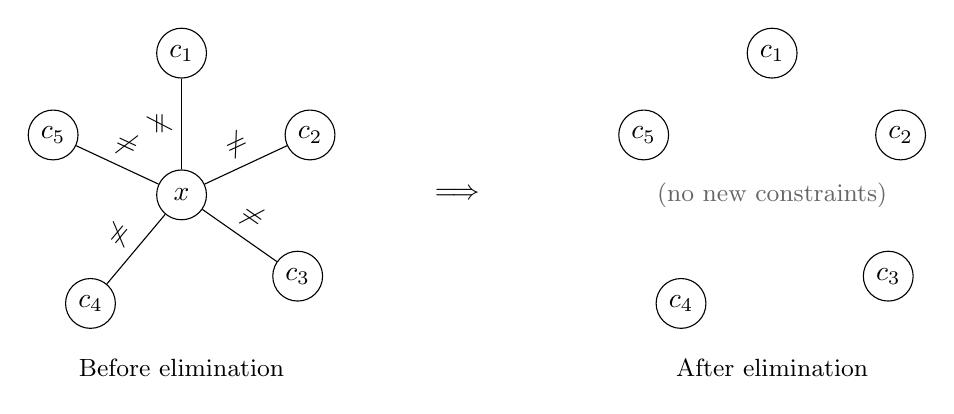
\begin{tikzpicture}[>=Latex]
    \begin{scope}[xshift=-2.5cm]
      \node[graphnode] (x2) at (0,0) {$x$};
      \foreach \angle/\name in {90/c_1,25/c_2,-35/c_3,-130/c_4,155/c_5} {
        \node[graphnode] (\name) at (\angle:1.8) {$\name$};
        \draw[-] (x2) -- node[midway,sloped,above] {$\neq$} (\name);
      }
      \node[font=\small,align=center] at (0,-2.2) {Before elimination};
    \end{scope}

    \node at (1,0) {$\Longrightarrow$};

    \begin{scope}[xshift=5cm]
      \node[graphnode,opacity=0] (x3) at (0,0) {$x$};
      \foreach \angle/\name in {90/c_1,25/c_2,-35/c_3,-130/c_4,155/c_5} {
        \node[graphnode] (\name p) at (\angle:1.8) {$\name$};
      }
      \node[font=\small,color=black!60] at (0,0) {(no new constraints)};
      \node[font=\small,align=center] at (0,-2.2) {After elimination};
    \end{scope}
  \end{tikzpicture}
\end{figure}

The OxCaml mode solver has constraints of the form $x \leq G(y)$ where $G$ are modalities with left adjoints. Like the interval constraints we considered above, these constraints can be solved in polynomial time using variable elimination, and for the same reason.

\subsection{Which constraints can be solved by elimination?}

For a set of constraints to be solvable by elimination, we need that the original problem has a solution iff the transformed problem has a solution. We will now analyze precisely when this property holds, and provide an easily checkable criterion for it.

Eliminating $x$ yields edges $R_{ij} = R_{i}^{\top} R_{0}^{\ast} R_{j}$ directed from $y_j$ to $y_i$ for all $i \geq j$, including self-loops $R_{ii}$.
If there were existing relations between the $y_i$ then we intersect them with these. Figure~\ref{fig:star-elim} illustrates the local transformation on the ``star'' centered at $x$.

\begin{figure}[ht]
  \centering
  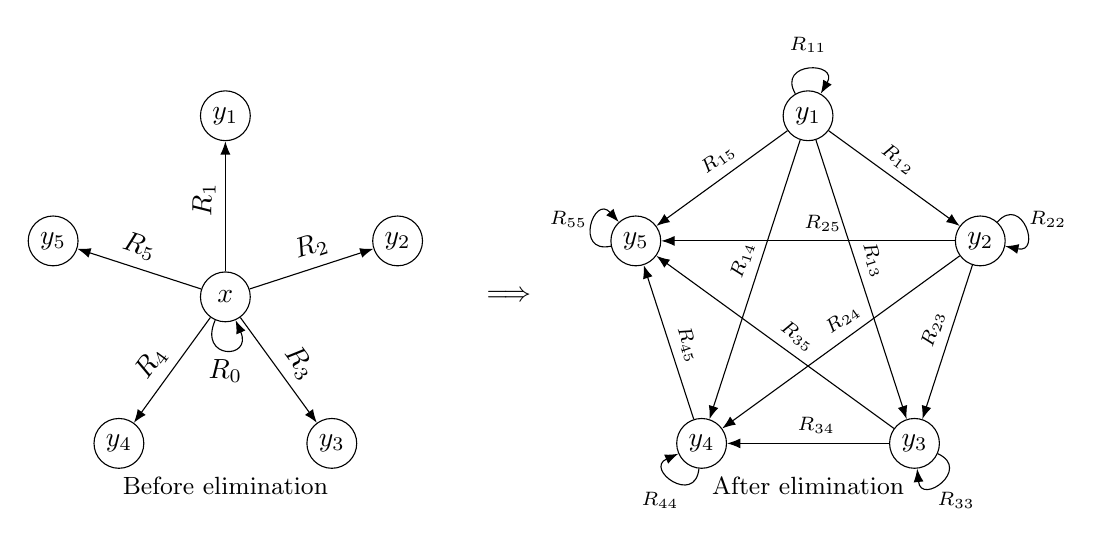
\begin{tikzpicture}[>=Latex]
    \begin{scope}[xshift=-3.2cm]
      \node[graphnode] (xbefore) at (0,0) {$x$};
      \foreach \idx/\angle in {1/90,2/18,3/-54,4/-126,5/162} {
        \node[graphnode] (yB\idx) at (\angle:2.3) {$y_{\idx}$};
        \draw[->] (xbefore) -- node[pos=0.55,above,sloped] {$R_{\idx}$} (yB\idx);
      }
      \draw[->] (xbefore) .. controls (-0.35,-0.8) and (0.35,-0.8) .. node[pos=0.5,below] {$R_{0}$} (xbefore);
      \node[font=\small] at (0,-2.4) {Before elimination};
    \end{scope}

    \node at (0.4,0) {$\Longrightarrow$};

    \begin{scope}[xshift=4.2cm]
      \foreach \idx/\angle in {1/90,2/18,3/-54,4/-126,5/162} {
        \node[graphnode] (yA\idx) at (\angle:2.3) {$y_{\idx}$};
        \draw[->] (yA\idx) .. controls +({\angle+30}:0.8) and +({\angle-30}:0.8) .. (yA\idx);
        \path (yA\idx) ++({\angle}:0.9) node[font=\scriptsize] {$R_{\idx\idx}$};
      }

      \foreach \i/\j in {5/4,5/3,5/2,5/1,4/3,4/2,4/1,3/2,3/1,2/1} {
        \draw[->] (yA\j) -- node[pos=0.45,above,font=\scriptsize,sloped] {$R_{\j\i}$} (yA\i);
      }

      \node[font=\small] at (0,-2.4) {After elimination};
    \end{scope}
  \end{tikzpicture}
  \caption{Eliminating $x$ in the radial layout yields edges $R_{ji}$ (with $R_{ji} \stackrel{\mathrm{def}}{=} R_{j}^{\top} R_{0}^{\!*} R_{i}$) directed from $y_j$ to $y_i$ for all $i \geq j$, as well as self loops $R_{ii}$.}
  \label{fig:star-elim}
\end{figure}

\textbf{The key question is: for which families of relations $\RelSet$ does this algorithm work?}

\paragraph{Answer.}
Intuitively, the elimination step is sound if every time we eliminate a variable $x$, the
constraints we generate between its neighbors are ``complete'': any solution of the
projected constraints on the neighbors can be extended to a value of $x$.
The obstruction is exactly the phenomenon we saw with $\neq$-constraints: locally
consistent projections need not extend.

We now characterize when elimination is complete.

\subsection{Closure and slices}

Fix a finite domain $V$ and a finite family of binary relations
$\RelSet \subseteq \mathcal{P}(V \times V)$.
The elimination algorithm only ever uses relations obtained from $\RelSet$ by:
\begin{itemize}
  \item composition: $RS = \{(a,c) \mid \exists b.\ (a,b)\in R \land (b,c)\in S\}$,
  \item intersection: $R \cap S$,
  \item converse: $R^{\top} = \{(b,a) \mid (a,b)\in R\}$,
  \item restriction to the diagonal (from self-loops): $R^{\ast} = \{(a,a) \mid (a,a)\in R\}$.
\end{itemize}
Let $\Cl(\RelSet)$ be the smallest set of relations containing $\RelSet$ and closed under
these four operations.

For a relation $R \in \Cl(\RelSet)$ and an element $b \in V$ we write:
\[
  R[\_,b] \;=\; \{ a \in V \mid (a,b)\in R \}
  \qquad\text{and}\qquad
  R[a,\_] \;=\; \{ b \in V \mid (a,b)\in R \}
\]
for its \emph{column} and \emph{row} slices.
These are exactly the unary constraints on $x$ induced by fixing the other endpoint.

Let $\mathcal{F}$ be the family of all such slices:
\[
  \mathcal{F}
  \;=\;
  \{\, R[\_,b], R[a,\_] \mid R \in \Cl(\RelSet),\ a,b\in V \,\}
  \;\subseteq\; \mathcal{P}(V).
\]

Because $\Cl(\RelSet)$ is closed under intersection, so is $\mathcal{F}$:
for any $A,B\in\mathcal{F}$ there exists $C\in\mathcal{F}$ with $C = A\cap B$.
This intersection-closure is crucial below.

\subsection{A Helly-style condition}

The key combinatorial property is a Helly-type condition on $\mathcal{F}$.

\begin{definition}[Helly-2 for slices]
We say that $\RelSet$ has the \emph{Helly-2 slice property} if the following holds:

For every finite subfamily $\{F_1,\dots,F_k\}\subseteq\mathcal{F}$,
if all pairwise intersections are non-empty,
\[
  F_i \cap F_j \neq \varnothing \quad\text{for all } i\neq j,
\]
then the total intersection is non-empty,
\[
  \bigcap_{i=1}^k F_i \neq \varnothing.
\]
\end{definition}

Because $\mathcal{F}$ is intersection-closed, this is equivalent to the absence of a
\emph{bad triple}:

\begin{lemma}[Triples suffice for intersection-closed families]
\label{lem:helly-triples}
Assume $\mathcal{F}$ is closed under intersection.
Then $\mathcal{F}$ has the Helly-2 slice property if and only if there do not exist
$A,B,C \in \mathcal{F}$ such that
\[
  A\cap B \neq \varnothing,\quad
  B\cap C \neq \varnothing,\quad
  C\cap A \neq \varnothing,\quad
  A\cap B\cap C = \varnothing.
\]
\end{lemma}

\begin{proof}
($\Rightarrow$) Immediate: such a triple would violate Helly-2.

($\Leftarrow$)
Suppose Helly-2 fails. Pick a counterexample
$\{F_1,\dots,F_m\}\subseteq\mathcal{F}$ of minimal size:
all pairs intersect, but $\bigcap_i F_i = \varnothing$.
Since $\mathcal{F}$ is intersection-closed, for each $i\ge2$ the set
$A_i := F_1\cap F_i$ lies in $\mathcal{F}$, is non-empty, and
$\bigcap_{i=2}^m A_i = \bigcap_{i=1}^m F_i = \varnothing$.
If some $A_i\cap A_j$ were empty, then
$F_1,F_i,F_j$ would form a bad triple.
Otherwise $\{A_2,\dots,A_m\}$ is a smaller counterexample, contradicting minimality.
\end{proof}

Thus in our setting we can detect failure of the Helly-2 slice property by a finite search
for such bad triples among slices in $\Cl(\RelSet)$.

\subsection{Correctness of elimination}

We now state the main correctness criterion.

\begin{theorem}[Characterization of admissible constraint families]
\label{thm:elimination-correct}
Let $V$ be finite and $\RelSet \subseteq \mathcal{P}(V\times V)$.
Consider the following variable-elimination algorithm:
at each step, pick a variable $x$, and for every two neighbors
$y_i \xleftarrow{R_i} x \xrightarrow{R_j} y_j$
insert the composed edge
\(
  y_i \xleftarrow{R_i R_0^\ast R_j} y_j
\)
(where $R_0^\ast$ is the current self-loop on $x$, possibly $\mathrm{Id}$),
intersecting with any existing edge between $y_i$ and $y_j$,
then delete $x$.
If at any point a self-loop on some variable becomes empty on the diagonal
(i.e. forbids all $(a,a)$), report unsatisfiable.

Then the following are equivalent:
\begin{enumerate}
  \item For every finite constraint graph over $\RelSet$, this elimination algorithm
        decides satisfiability correctly: the final instance is satisfiable
        iff the original instance is satisfiable.
  \item $\RelSet$ has the Helly-2 slice property.
\end{enumerate}
\end{theorem}

\begin{proof}[Proof sketch]
$(2) \Rightarrow (1)$ (\emph{completeness of elimination}).
It is enough to show that a \emph{single} elimination step is complete, and then argue by
induction on the number of variables.

Consider eliminating $x$ from its star.
Fix an assignment to the neighbors $\{y_i\}$ that satisfies all constraints
generated by the algorithm between the $y_i$.
For each incident edge, this assignment induces a slice
$S_i \in \mathcal{F}$ of admissible values for $x$
(e.g., for $y_i \xrightarrow{R_i} x$ with $y_i$ fixed to $b_i$ we get
$S_i = R_i[\_,b_i]$).
By construction, every binary constraint added between $y_i$ and $y_j$ enforces that
$S_i$ and $S_j$ intersect: if they did not, the corresponding composed relation would
have removed the chosen pair $(b_i,b_j)$.
Hence the family $\{S_i\}$ is pairwise-intersecting.
By the Helly-2 slice property,
\(
  \bigcap_i S_i \neq \varnothing.
\)
Picking any $a$ in this intersection and setting $x:=a$ extends the neighbor assignment to
a full solution of the original constraints around $x$.
Inductively, every model of the final instance lifts to a model of the original one.

Soundness of the algorithm (it never introduces spurious solutions) holds because every
new edge relation is logically implied by the existence of an intermediate $x$ satisfying
its incident constraints.

$(1) \Rightarrow (2)$ (\emph{necessity}).
Assume the Helly-2 slice property fails.
By Lemma~\ref{lem:helly-triples} and intersection-closure, there exist
$S_1,S_2,S_3 \in \mathcal{F}$
with all pairwise intersections non-empty but empty triple intersection.
By definition of $\mathcal{F}$, we can realize each $S_i$ as the admissible values for
some variable $x$ given a fixed neighbor $y_i$ and a relation $R_i \in \Cl(\RelSet)$.
We construct a constraint star with center $x$ and leaves $y_1,y_2,y_3$ so that, for the
chosen values of the $y_i$, the corresponding slices are precisely $S_i$.
By pairwise intersection, every pair of leaves admits a value of $x$;
hence the elimination algorithm, which only asserts pairwise compositions,
accepts this partial assignment to $y_1,y_2,y_3$.
But by emptiness of $S_1\cap S_2\cap S_3$, no value of $x$ satisfies all three
constraints simultaneously, so the original instance is unsatisfiable.
Thus elimination is not complete, contradicting~(1).
\end{proof}

\begin{corollary}[Finite check]
\label{cor:finite-check}
For finite $V$, the Helly-2 slice property for $\RelSet$ is decidable:
\begin{enumerate}
  \item compute $\Cl(\RelSet)$ (finite);
  \item form all slices $R[\_,b], R[a,\_]$;
  \item check that no triple of slices has non-empty pairwise intersections and empty
        triple intersection.
\end{enumerate}
If no such triple exists, variable elimination as above is sound and complete for all
constraint graphs over $\RelSet$.
\end{corollary}

In particular, difference constraints and the OxCaml-style modal constraints
$x \leq G(y)$ with adjoints fall into this framework:
their induced slices are (discrete) intervals, which satisfy Helly-2, so elimination is
complete.
By contrast, $\neq$-constraints generate non-convex slices, violate Helly-2, and are
correctly rejected by this criterion.


\section{Solver Architecture}

\section{Open Questions}

\end{document}
